\subsection{Architecture du programme}
Pour notre application, nous avons adopté l’architecture \textbf{MVC} (Modèle Vue Contrôleur).
Ainsi, nous avons dédié quelques packages au modèle qui gère toute la logique métier, un package contenant la vue (interface graphique), et des événements capturés sur la vue pour agir sur le modèle (contrôleur). Le modèle est complètement indépendant de la vue, et la vue représente les données du modèle. Nous avons appliqué au MVC un observer pattern. Les classes du modèle (celles pour lesquelles c'est utile) implémentent donc une interface observable et celles de la vue une interface observer pour écouter sur la vue.
\begin{itemize}
\item \textbf{app} : ce package contient toutes les classes liées à la logique du jeu, notamment les classes \texttt{Game} et \texttt{Generator}, ainsi que la classe \texttt{GeneratorThread} pour la gestion des thread
\item \textbf{constants} : ce package contient toutes les constantes utilisées dans notre programme, telles que les constantes associées au type de voisinage du jeu et les constantes associées à la  règle classique  du jeu de la vie. regroupe les classes "NeighborsType" et "Rules"
\item \textbf{modele} : ce package contient toutes les classes liées  à la gestion des données. En plus de contenir les classes "Cellule","Grid","Position ,le package modele contient deux sous-packages :
\begin{itemize}
\item \textbf{hashlife} : ce sous-package contient toutes les parties liées à l'implémentation de Hashlife, une technique avancée pour accélérer les calculs du jeu de la vie , il contient la classe "Hashlife" et "QuadNode"
\item \textbf{rule}:ce sous-package contient toutes les parties liées à l'implémentation des règles classiques du jeu de la vie ainsi que des règles personnalisables par l'utilisateur. Il contient des classes pour la définition et l'application des règles, ainsi que pour la gestion des règles personnalisées définies par l'utilisateur.il contient les classes : "Rule","RuleMulttF",
"RuleRange","RuleFormat"
\end{itemize}
\item \textbf{tests} : ce package contient toutes les classes de tests nécessaires pour notre projet, pour assurer le bon fonctionnement de toutes les fonctionnalités du jeu.
\item \textbf{image} : ce package contient toutes les images utilisées dans notre interface homme-machine, telles que les icônes de boutons et les images de fond d'écran.
\item \textbf{patterns} : ce package contient tous les fichiers utilisés pour générer les patterns, qui sont des motifs prédéfinis de cellules utilisés dans le jeu.
\item\textbf{Util} : Le package Util contient toutes les classes liées aux événements, comme les
écouteurs d’événements. Ces classes sont utilisées pour écouter les événements
déclenchés par l’utilisateur, comme le clic de la souris. Les écouteurs sont ensuite utilisés pour déclencher des actions spécifiques dans le jeu,elle contient les classes "AbstractListenableModel","ListenableModel" et "ListeningModel"
\item\textbf{views} : Le package Views contient toutes les classes liées à l’interface utilisateur.
C’est là que nous avons stocké toutes les classes qui gèrent l’affichage des
éléments graphiques, comme les fenêtres de dialogue et la grille du jeu. Les
classes de ce package utilisent les classes du package modele pour récupérer les
données liées au jeu et les afficher à l’utilisateur
\end{itemize}
 En organisant notre code de cette manière, nous avons pu séparer efficacement les différentes parties du programme et travailler de manière structurée.
\newpage
\begin{figure}[h]
		\centering
      \raggedright  
		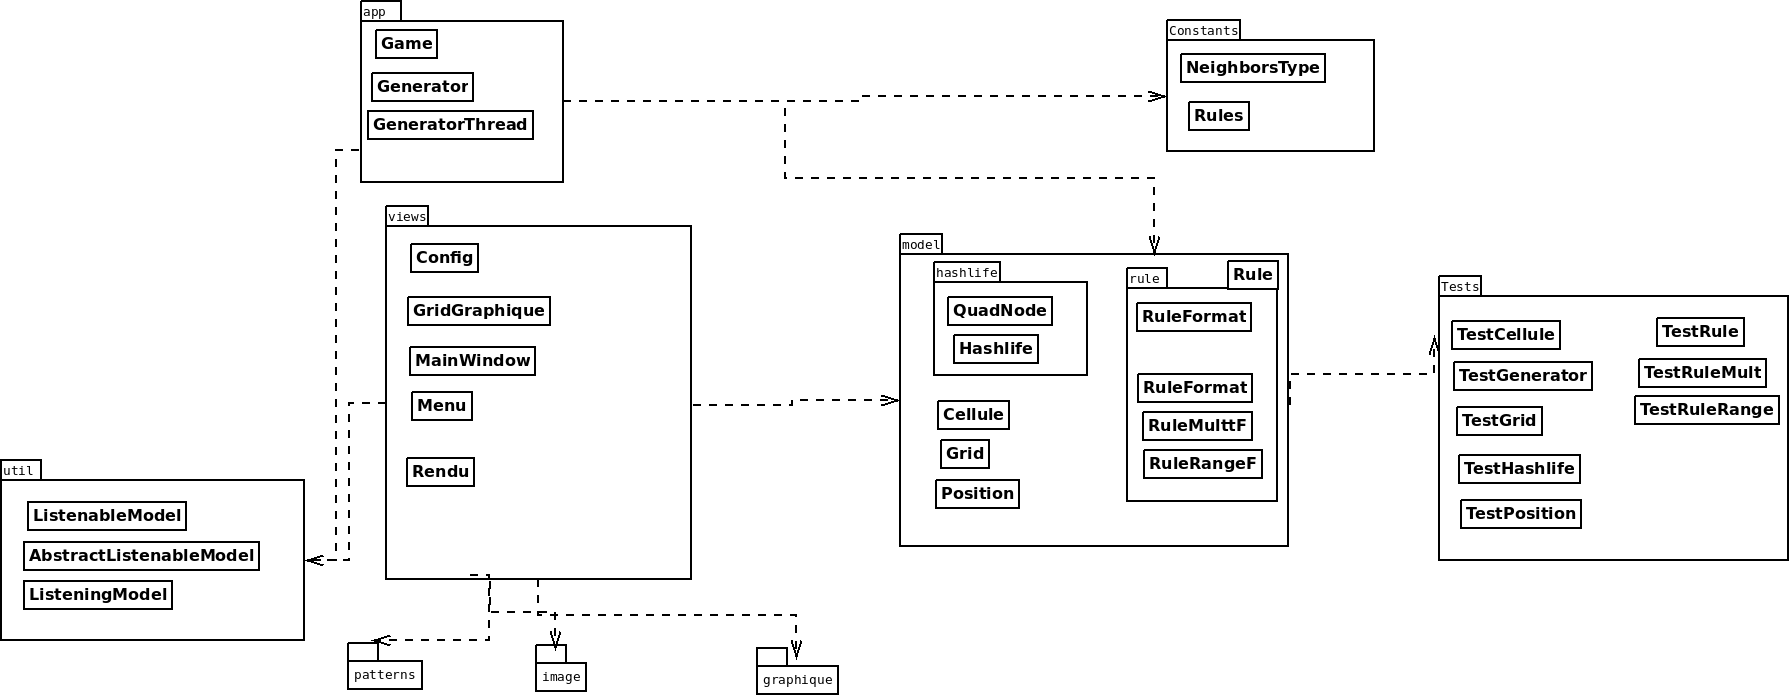
\includegraphics[width=16cm]{images/package.PNG}
	    \caption{Diagramme des packages }
\end{figure}
\newpage
\begin{figure}[h]
		\centering
      \raggedright   
		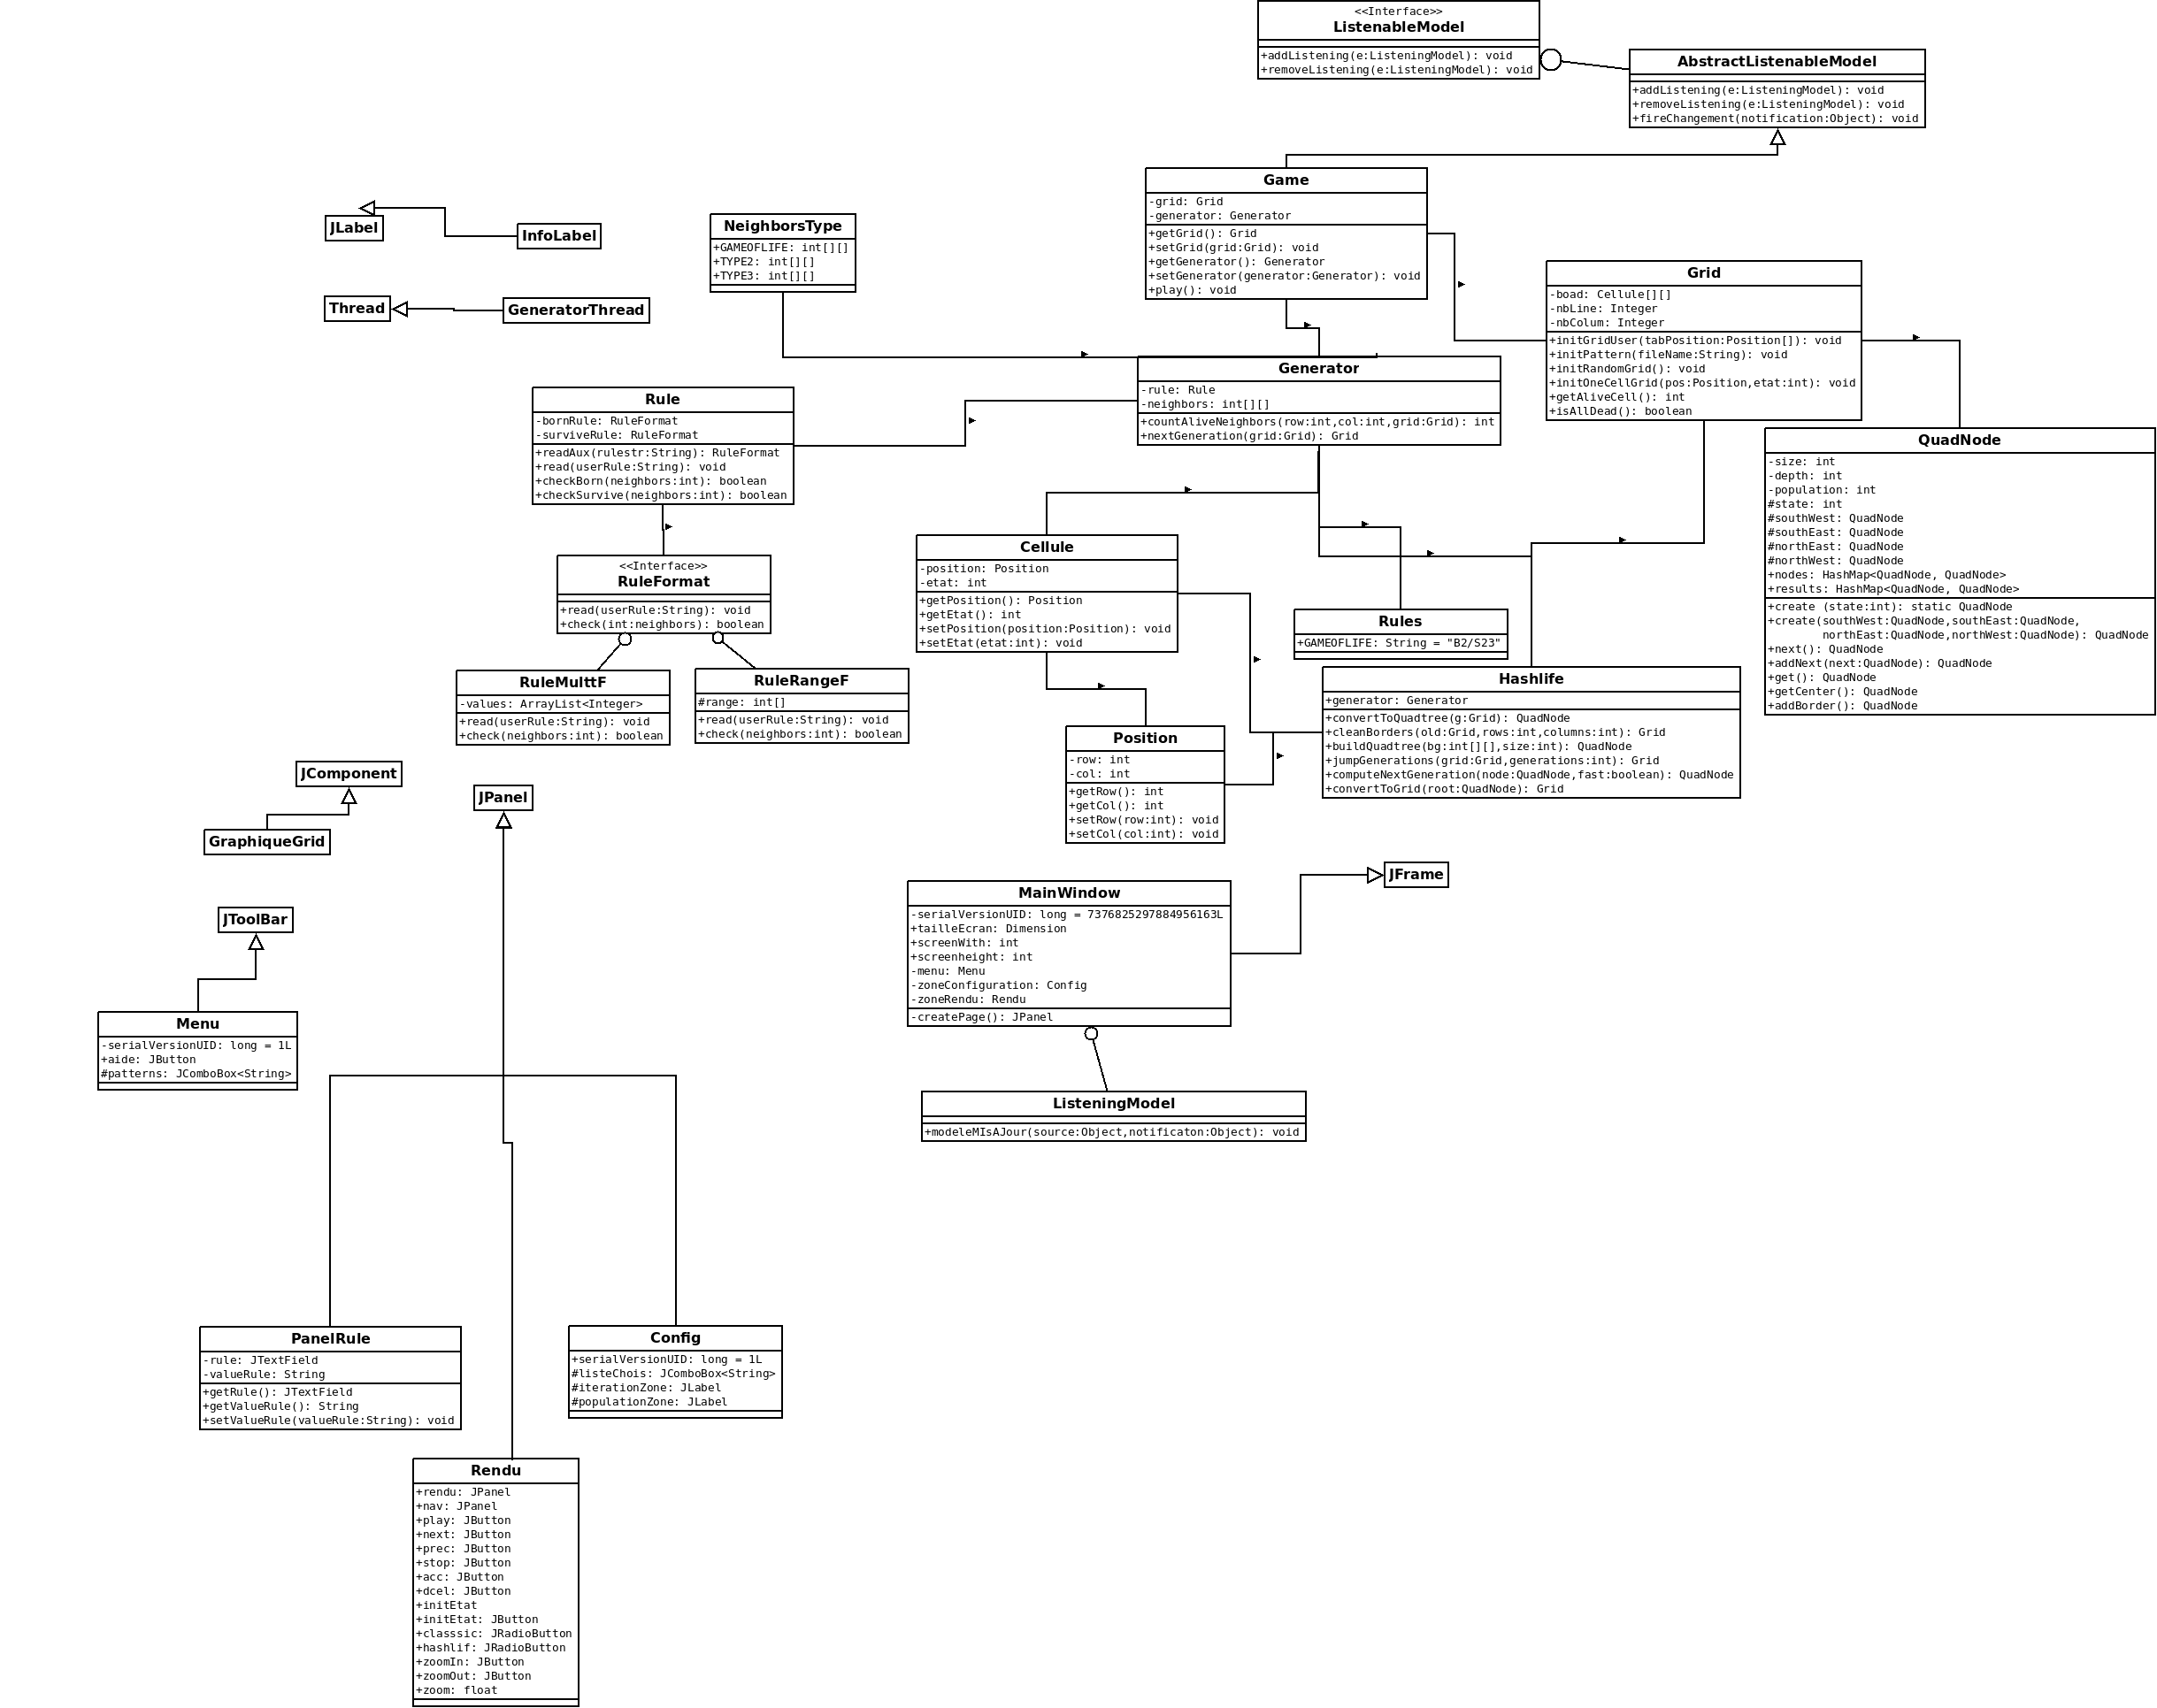
\includegraphics[width=17cm]{images/classes.png}
	    \caption{Diagramme des Classes }
\end{figure}